\documentclass[twoside,twocolumn,10pt]{article}
\usepackage{fancyhdr}
\usepackage{geometry}
\usepackage{abstract}
\usepackage{graphicx}
\usepackage{caption}
\usepackage{titlesec}
\usepackage{ragged2e}
\usepackage{amssymb}
\usepackage{parskip}
\usepackage{amsmath}
\usepackage{newtxtext}
\usepackage{booktabs}
\usepackage{array}

\setcounter{page}{1}

\newcolumntype{L}[1]{>{\raggedright\arraybackslash}p{#1}}
\newcolumntype{C}[1]{>{\centering\arraybackslash}p{#1}}
\newcolumntype{R}[1]{>{\raggedleft\arraybackslash}p{#1}}

\usepackage[font=footnotesize, labelfont=bf, justification=raggedright, format=plain]{caption}

\captionsetup[table]{labelsep=period, justification=raggedright}
\captionsetup[figure]{labelsep=period, justification=raggedright}

\usepackage[backend=bibtex,style=ieee]{biblatex}
\addbibresource{references.bib}
\defbibheading{bibliography}[\refname]{\section{\MakeUppercase{References}}}

\geometry{a4paper, left=0.8in, right=0.8in, top=1in, bottom=1in}
\setlength{\columnsep}{15pt}

\renewcommand{\abstractname}{\hspace{1.3em}\textbf{Abstract}}

\titleformat{\section}{\large\bfseries\uppercase}{\thesection.}{1em}{}
\titleformat{\subsection}{\normalfont\bfseries\flushleft}{\thesubsection.}{1em}{}
\titleformat{\subsubsection}{\normalfont\bfseries\itshape\flushleft}{\thesubsubsection}{1em}{}

\renewcommand{\abstractnamefont}{\normalfont\fontsize{14}{20}\bfseries}
\renewcommand{\absnamepos}{flushleft}
\renewcommand{\abstracttextfont}{\normalfont\fontsize{11}{13}\selectfont}

\newcommand{\keywordsname}{Keywords}
\newenvironment{keywords}
  {\par\noindent\hspace{2em}\textbf{\keywordsname:}}
  {\par}

\hyphenpenalty=10000
\exhyphenpenalty=10000
\sloppy

\pagestyle{fancy}
\fancyhf{}
\fancyhead[C]{\small Smart Email Prioritization}
\fancyhead[CE]{\small Tirumani et al. (2026)}
\fancyfoot[C]{\thepage}

% First-page header/footer: neutral course-project framing, not a real
% journal issue. Do not fill in ISSN/volume/received-revised-accepted
% metadata here -- this is a course project report, not a journal
% submission, and fabricating publication metadata would be misleading.
\fancypagestyle{firstpage}{
  \fancyhf{}
  \fancyhead[LO]{\small CS6140 -- Final Project Report}
  \fancyhead[RO]{\small Summer 2026}
  \fancyfoot[L]{\footnotesize Northeastern University, CS6140}
  \fancyfoot[R]{\footnotesize Code: \url{https://github.com/Shdityr/CS6140_email_priority}}
  \renewcommand{\headrulewidth}{0.4pt}
  \renewcommand{\footrulewidth}{0.4pt}
}

\title{\fontsize{16}{20}\selectfont\textbf{Smart Email Prioritization}}
\author{
    \fontsize{12}{14}\selectfont
    Vignesh Tirumani\textsuperscript{1}, Sathvik Reddy Cheruku\textsuperscript{1}, Zhidian Wang\textsuperscript{2}\\[1ex]
    \fontsize{11}{13}\selectfont
    \textsuperscript{1}MS in Artificial Intelligence, Northeastern University, Portland, Maine, USA\\
    \textsuperscript{2}MS in Artificial Intelligence, Northeastern University, Silicon Valley, California, USA
}
\date{}

\begin{document}

\twocolumn[
\begin{@twocolumnfalse}
\vspace{-0.5cm}
\raggedright

{\fontsize{11}{13}\selectfont{Final Project Report}}
\vspace{-0.8cm}

\maketitle
\thispagestyle{firstpage}

\begin{abstract}
\fontsize{11}{13}\selectfont
\vspace{1em}
\justifying
Email inbox overload is a well-known productivity problem, and unlike spam filtering, what counts as a ``priority'' email is inherently personal rather than universal. We build a fully local, privacy-preserving email-priority classifier centered on a small, hand-designed 18-feature logistic regression, initialized from a hand-tuned cold-start prior and personalized per user via online gradient descent anchored to that prior. Using three real, independently collected and labeled Gmail datasets, we empirically compare this approach against two alternatives we also implemented: a variant that mines additional term features from the public Enron corpus via TF-IDF, and a general-purpose large language model (Claude Haiku 4.5) prompted with no hand-designed features at all. We find that the hand-crafted model outperforms both alternatives on measured, held-out accuracy, while remaining fully explainable and free of third-party API cost; the Enron-mined vocabulary overfits to corpus-specific employee names rather than a transferable notion of importance, and the LLM alternative, while achieving perfect recall, trades away substantial precision and carries a real, measured per-classification dollar cost and latency. We further show that online personalization itself is not universally beneficial: it produces a reproducible positive accuracy lift on one dataset and a reproducible negative lift on a smaller one, most likely because too little accumulated feedback gives the prior-anchored gradient descent no reliable signal to work from. These findings suggest that both a ``one-size-fits-all'' prior and an assumption that personalization always helps are unsafe defaults for personal, privacy-sensitive classification tasks with small per-user data.

\vspace{-0.1cm}
\noindent\textbf{Keywords}
 Email prioritization, personalization, online learning, logistic regression, large language models, feature engineering.

\end{abstract}

\vspace{1cm}
\end{@twocolumnfalse}
]

\fontsize{12}{14}\selectfont

\section{Introduction}

Inbox overload is a well-documented productivity problem: users receive a mix of high-priority mail (from managers, collaborators, and institutions) and low-priority mail (marketing, automated notifications, digests), with no reliable automatic way to separate them. Unlike spam filtering, where ``unwanted'' is close to a universal category, email \emph{priority} is inherently personal: a newsletter one person deletes on sight is exactly what another person opens first, so a system that gets priority right must adapt to the individual rather than apply a fixed global rule.

There is no public, pre-labeled dataset for this task, since email content and a person's private judgment about what matters to them are both sensitive. We therefore built our own: each team member exported and hand-labeled a batch of their own real Gmail inbox with a purpose-built extraction tool, marking every message Keep (something they would want surfaced) or Skip (everything else). This binary decision is the target variable for the whole project. We supplement it with the public Enron email corpus~\cite{klimt2004enron} as an auxiliary, differently-purposed dataset (Section~\ref{sec:data}).

This kind of data surfaces three challenges beyond a conventional fixed-label dataset. First, ``ground truth'' is subjective and non-transferable: a prior tuned on one person's labels can fail completely on another's (Section~\ref{sec:analysis}). Second, realistic per-user data volume is small -- our three datasets range from 50 to 200 emails, well below typical supervised-learning benchmarks, with class balance varying by person. Third, privacy constraints limit what can be measured: the extraction tool never captures full message bodies, only subject lines, short snippets, and structural header metadata, so every feature must be derivable from that limited surface.

We built a lightweight, fully local email-priority classifier that (a) starts from a hand-tuned general-purpose baseline requiring no user data, and (b) adapts to an individual's preferences from their own feedback, entirely on the user's own machine, with no email content sent to a third-party AI service and no Gmail credentials leaving it.

\section{Proposed Method: Overview}

Our method is a single logistic regression over an 18-dimensional, hand-designed feature vector (Section~\ref{sec:method}), initialized to a hand-tuned ``cold-start'' prior and personalized per user via online gradient descent toward that prior. We chose this over two alternatives we also built and empirically measured rather than assumed superior: (1) an earlier iteration mining 15 term features from Enron via TF-IDF, found to memorize corpus-specific vocabulary (largely Enron employees' first names) rather than a generalizable notion of importance, and dropped as a training source (Section~\ref{sec:analysis}); and (2) a general-purpose LLM (Claude Haiku 4.5) with no hand-designed features at all, measured to be less accurate on our real data and to carry a real per-classification dollar cost and latency (Section~\ref{sec:results}). The hand-crafted approach suits our setting -- small per-user data, a need to explain decisions, fully local zero-marginal-cost inference -- at the cost of the richer pattern-matching a learned text representation could offer.

\section{Related Work}

\textbf{Personalized email importance ranking.} The closest prior work is Aberdeen, Pacovsky, and Slater's account of Gmail Priority Inbox~\cite{aberdeen2010gmail}, which frames ``importance'' as a personalized, per-user online-learning problem over hand-designed social, content, and thread features -- the same overall shape as our system. Yoo, Yang, Lin, and Moon~\cite{yoo2009mining} extend this by mining a user's social network alongside content features and semi-supervised clustering. Yoo, Yang, and Carbonell~\cite{yoo2011modeling} frame prioritization as ordinal classification and find a cascade of binary classifiers beats ordinal regression. All three assume a large user population and hundreds of behaviorally-mined features; we instead use 18 features computable from one user's own mailbox and Sent folder, with no cross-user aggregation -- trading population-scale signals for zero centralized infrastructure (Section~\ref{sec:analysis}).

\textbf{Hand-crafted-feature spam and junk-mail filtering.} Sahami, Dumais, Heckerman, and Horvitz's Bayesian junk-mail filter~\cite{sahami1998bayesian} combines naive Bayes with hand-crafted non-textual features (subject phrases, sender domain, direct addressing) -- the philosophy our \texttt{is\_bulk\_header}, \texttt{system\_sender}, and \texttt{direct\_to} features descend from, applied to priority ranking rather than spam/ham. Apache SpamAssassin~\cite{spamassassin} extends this with a large hand-maintained rule set; several of our features are conceptually similar header rules, applied per-mailbox rather than globally. Klimt and Yang's Enron release~\cite{klimt2004enron} both supplied our auxiliary test set (Section~\ref{sec:data}) and the baseline we build on in our TF-IDF exploration (Section~\ref{sec:analysis}).

\textbf{Linear models for text classification.} Joachims~\cite{joachims1998text} shows linear classifiers over sparse, high-dimensional bag-of-words features perform strongly because text classification has many weakly-informative features and few irrelevant ones -- motivating our own choice of logistic regression (Section~\ref{sec:method}), and explaining a negative result in Section~\ref{sec:analysis}: a vocabulary mined once from Enron does not generalize across mailboxes the way Joachims's classifier generalized within one fixed corpus, since a different user's vocabulary leaves a fixed-vocabulary model nothing left to adapt.

Our contribution is not a new algorithm but a specific design point -- a linear, hand-crafted-feature, per-user-online-learned classifier for tens to hundreds of labels and zero centralized infrastructure -- validated against both a corpus-mined-feature variant and a general-purpose LLM on real personal inboxes (Sections~\ref{sec:analysis}, \ref{sec:results}).

\section{Related Implementations}

Our primary dataset (team-collected real Gmail exports) is private and not published on Kaggle, so we compare instead against public Kaggle work on the Enron corpus~\cite{klimt2004enron}, which we also use as an auxiliary dataset (Section~\ref{sec:data}). Three representative examples:

\begin{enumerate}
\item \textbf{Enron Email Classification}~\cite{adrian_enron_kaggle}: TF-IDF vectorization followed by classical supervised classifiers, in the same spirit as our own now-abandoned TF-IDF exploration (Section~\ref{sec:analysis}).
\item \textbf{Enron email classification using machine learning}~\cite{ankur_enron_kaggle}: a similar bag-of-words / TF-IDF representation with standard classifiers (Naive Bayes, logistic regression, tree-based models).
\item \textbf{Spam email classifier from Enron dataset}~\cite{solano_enron_kaggle}: a labeled Enron-derived spam/ham split treated as binary TF-IDF text classification.
\end{enumerate}

All three train once on a static vocabulary and static labels and report a single held-out accuracy. Our system differs in two respects: we do not use Enron as a training source in the live system at all (Section~\ref{sec:analysis}), since vocabulary mined from any one static corpus encodes that corpus's own properties (here, specific employees' names) rather than a transferable notion of importance; and our target is not a one-time classification of a fixed corpus but a continuously personalizing model for one individual mailbox, refit online from that person's own feedback (Section~\ref{sec:method}) -- a use case these fixed-corpus notebooks are not designed for.

\section{Data Analysis}
\label{sec:data}

\textbf{Primary data -- team-collected real Gmail exports.} Each team member labeled a batch of their own real inbox with a purpose-built extraction tool: every email defaults to Skip, and the labeler marks Keep for anything they would genuinely want surfaced, or Skip (privacy) for anything they do not want counted or shared. The exporter stores only the subject line, sender, a short snippet, and structural header fields -- never full email bodies or credentials. Three datasets were collected this way (Table~\ref{tab:datasets}), all skewed toward Skip rather than balanced (19--28\% Keep), which is itself an important property of this kind of data: a real inbox has no guarantee of balanced classes.

\begin{table}[h]
\centering
\caption{Team-collected real Gmail datasets.}
\label{tab:datasets}
\resizebox{\columnwidth}{!}{%
\begin{tabular}{@{}lcccc@{}}
\toprule
\textbf{Tester} & \textbf{Exported} & \textbf{Usable} & \textbf{Keep} & \textbf{Skip} \\
\midrule
Zhidian & 200 & 193 & 54 & 139 \\
Vignesh & 60  & 50  & 13 & 37  \\
Sathvik & 100 & 94  & 18 & 76  \\
\bottomrule
\end{tabular}%
}
\end{table}

\textbf{Auxiliary data -- the Enron email corpus~\cite{klimt2004enron}.} Enron is a public collection of roughly 500{,}000 real corporate emails released during the Federal Energy Regulatory Commission's investigation into the Enron Corporation. It carries no priority labels, so we generated them heuristically from the folder a message was filed into: \texttt{sent}/\texttt{sent\_items}/\texttt{\_sent\_mail} (the employee chose to respond or act) were labeled Keep, and \texttt{deleted\_items}/\texttt{all\_documents}/\texttt{discussion\_threads} were labeled Skip, giving 30{,}000 heuristically labeled rows (15{,}000 per class) after capping for balance.

\textbf{Feature formulas.} Each of the 18 features is a plain scalar computed from the message text, sender string, or structural header fields -- no learned embeddings. Representative formulas from \texttt{feature\_vector()}: the shouting-subject signal is $\text{exclaim}=1$ if the subject and snippet together contain two or more exclamation marks (counting both the ASCII ``!'' and its full-width counterpart, U+FF01, used in Chinese text) else $0$; the business-hours signal is $\text{business\_hours}=1$ if the message's \texttt{Date} header hour (sender's own offset) falls in $[9,18)$ else $0$; the one online-learned feature, sender history, is $\text{sender\_hist} = (\text{keep\_count}/\text{total\_count}) - 0.5$ for that sender within the labeled examples seen so far, centered at $0$ for an unseen sender.

\textbf{Per-feature activation, Enron cold-start check.} Figure~\ref{fig:feature-activation} plots the mean activation of each of the 17 non-bias features on all 30{,}000 Enron-labeled rows, split by class, computed with no training (the live hand-tuned \texttt{PRIOR\_WEIGHTS} only). \texttt{many\_recipients} (0.077 Keep vs. 0.204 Skip), \texttt{question\_mark} (0.188 vs. 0.148), \texttt{has\_url} (0.028 vs. 0.057), and \texttt{business\_hours} (0.361 vs. 0.303) all separate in the direction their hand-tuned weight assumes. \texttt{personalized\_greeting} separates in the \emph{wrong} direction (0.001 vs. 0.026) -- a direct consequence of Enron's Keep class being the employee's own \emph{sent} mail rather than \emph{received} mail. Five features -- \texttt{has\_attachment}, \texttt{is\_bulk\_header}, \texttt{is\_reply\_thread}, \texttt{sender\_hist}, \texttt{reciprocal\_sender} -- show essentially zero activation in both classes on this Enron release: this specific 2015 export of the corpus strips MIME/threading/bulk-mail headers entirely, so this is a data-availability limitation of this particular Enron release, not a bug in our feature code.

\begin{figure}[h]
\centering
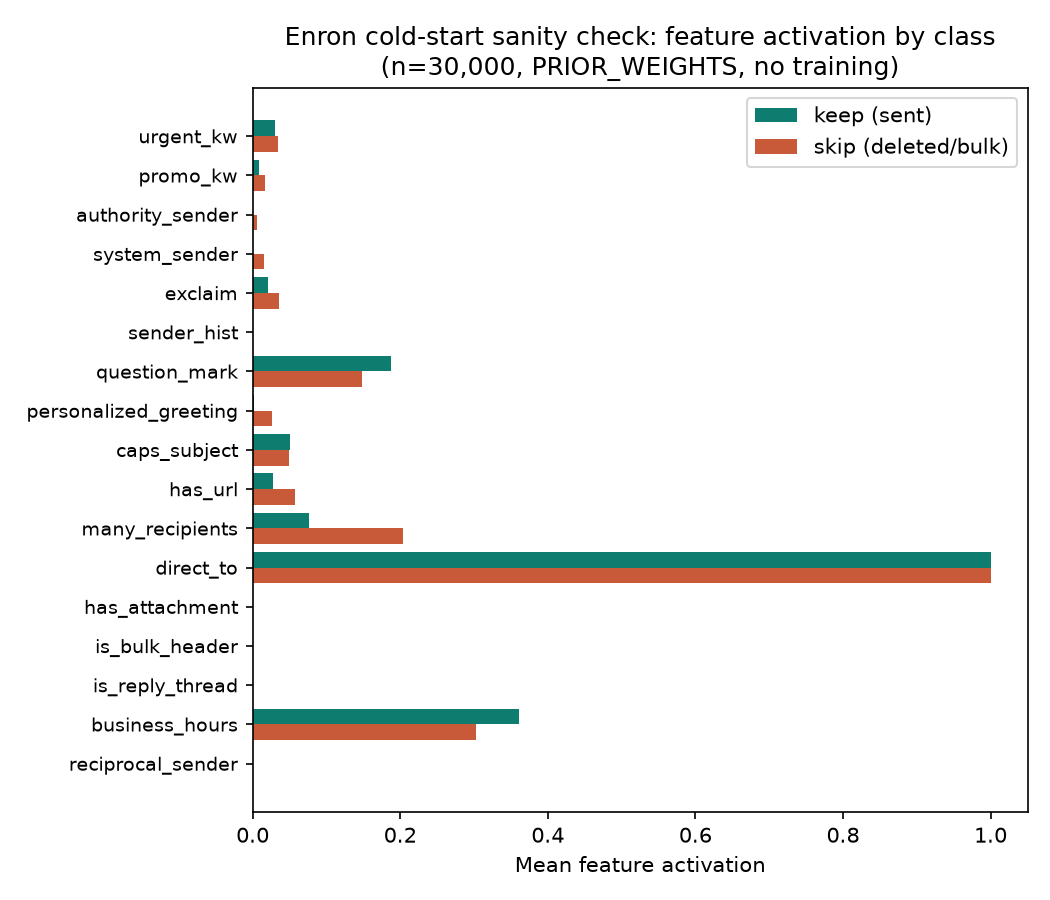
\includegraphics[width=0.5\textwidth]{figures/feature_activation.png}
\caption{Mean activation of each non-bias feature, keep (employee's own sent mail) vs. skip (deleted/bulk mail), across all 30{,}000 Enron heuristically labeled rows, using the live hand-tuned prior with no training.}
\label{fig:feature-activation}
\end{figure}

\section{Proposed Method: Algorithm Details}
\label{sec:method}

The classifier is a logistic regression over the 18-dimensional feature vector $\mathbf{x}$ described in Section~\ref{sec:data}, with weight vector $\mathbf{w}$ (\texttt{PRIOR\_WEIGHTS} as the untrained starting point). Given $\mathbf{x}$, the model computes a linear score and probability

\begin{align}
z &= \mathbf{w} \cdot \mathbf{x} \\
p &= \sigma(z) = \frac{1}{1+e^{-z}}
\end{align}

predicting Keep when $p > 0.5$.

\textbf{Feature design (18 features in two generations).} Generation 1 (7 features) contributes keyword lists for urgency and promotion, sender-string heuristics for authority (\texttt{authority\_sender}) and bulk senders (\texttt{system\_sender}), a shouting-subject heuristic, a constant \texttt{bias}, and \texttt{sender\_hist} -- the only feature computed from the user's own feedback history rather than the message itself. Generation 2 (11 features) adds text-only signals (question marks, personalized greetings, capitalized subjects, URLs) and header/structural signals parsed from real Gmail/IMAP headers: recipient count (\texttt{many\_recipients}), whether the user is a direct recipient (\texttt{direct\_to}), attachments, reply-thread markers (\texttt{is\_reply\_thread}), business hours, and \texttt{is\_bulk\_header} (RFC-compliance headers such as \texttt{List-Unsubscribe} or \texttt{Auto-Submitted}, more reliable than guessing bulk-ness from body keywords). A relationship signal, \texttt{reciprocal\_sender}, is computed from a one-time IMAP scan of the user's Sent folder at fetch time.

\textbf{Cold-start prior.} All 18 features carry a hand-tuned initial weight (\texttt{PRIOR\_WEIGHTS}), representing a reasonable general-purpose baseline before any user feedback exists -- for example, a strong negative weight on \texttt{is\_bulk\_header} and a strong positive weight on \texttt{sender\_hist} -- subsequently adjusted based on empirical testing against real labeled data (Section~\ref{sec:analysis}).

\textbf{Online personalization update.} On every classification request, the backend receives the complete history of labels the user has given so far and refits the model from the prior over $E=25$ epochs of full-batch gradient descent. For each labeled example $(\mathbf{x}, y)$ with $y \in \{0,1\}$, the per-step weight update is

\begin{align}
p &= \sigma(\mathbf{w}\cdot\mathbf{x}) \\
\text{error} &= c_y\,(y - p), \quad c_y = \begin{cases} 2.0 & y=1 \\ 1.0 & y=0 \end{cases} \\
\text{grad}_k &= \text{error}\cdot x_k - \lambda\,(w_k - w^0_k) \\
w_k &\leftarrow w_k + \eta \cdot \text{grad}_k
\end{align}

with learning rate $\eta = 0.3$, L2-toward-prior coefficient $\lambda = 0.08$, and $\mathbf{w}^0$ the untrained prior (\texttt{PRIOR\_WEIGHTS}, \texttt{L2\_TOWARD\_PRIOR}, \texttt{LEARNING\_RATE}, \texttt{KEEP\_CLASS\_WEIGHT} in \texttt{backend/app.py}). The $c_y$ term amplifies the gradient for Keep-labeled examples, deliberately trading some precision for recall since missing a genuinely important email is worse for this use case than occasionally surfacing an unimportant one. If fewer than two examples exist, or all examples share one label, training is skipped and the prior is used as-is, since gradient descent with a single class present would push every weight in one direction with no counterbalance.

\textbf{Why logistic regression suits this problem.} With only tens to a few hundred examples per user, a large or deep model would overfit; a linear model over a small, hand-designed feature space has far fewer parameters than examples, and -- as Joachims~\cite{joachims1998text} found for text classification -- linear models resist overfitting well when many features are individually weakly informative, which describes our design. The L2-toward-prior term anchors weights so a handful of contradictory labels cannot swing the decision boundary far from a sensible default. Every weight is also directly inspectable, so the system can report \emph{why} it made a call -- a requirement a black-box model would not satisfy as directly.

We separately built and measured a fundamentally different alternative: prompting a general-purpose LLM (\texttt{claude-haiku-4-5}) directly, with no hand-designed features, via a two-stage design -- one call summarizes labeled examples into a natural-language preference profile, and one batched call classifies a target batch against that profile using a forced tool call for reliable structured output (\texttt{backend/llm\_eval/claude\_classify.py}, using~\cite{anthropic_docs}). This mirrors production usage (one batch per request) rather than a round trip per email. Results and measured cost/latency are in Section~\ref{sec:results}.

\section{Analysis}
\label{sec:analysis}

\textbf{Why hand-designed structural features generalize and mined vocabulary does not.} We initially explored a third generation of features: refitting the seven Generation-1 features with 15 terms discovered by TF-IDF over Enron, producing a 22-feature model (\texttt{backend/enron/train\_prior.py}, kept in the repository but not loaded by the live system). Inspecting the retrained weights, rather than only the held-out accuracy, surfaced two problems we believe generalize to any single fixed training corpus. First, of the six retrainable Generation-1 features, \texttt{authority\_sender} and \texttt{system\_sender} were refit to $-2.91$ and $-3.02$ -- \texttt{authority\_sender}'s sign is the opposite of its design intent -- because Enron (corporate mail from the early 2000s) contains almost none of the keywords these features look for (``VP,'' ``director,'' ``no-reply''), so the regression's weight reflects noise, not a real contrast. Second, eight of the fifteen discovered terms (\texttt{lynn}, \texttt{michelle}, \texttt{rick}, \texttt{carson}, \texttt{monika}, \texttt{shelley}, \texttt{kayne}, \texttt{bailey}) are specific Enron employees' first names -- a real correlation in \emph{this} dataset that does not transfer to a mailbox where those names carry no meaning. Together with the accuracy gap alone (TF-IDF-only: 0.680 held-out; combined 22-feature model: 0.598, on a 25{,}500/4{,}500 split), this is why we replaced mined vocabulary with the 18 hand-designed structural features (Section~\ref{sec:method}): a bulk-mail header or recipient count means the same thing regardless of whose inbox it is, while a fixed mined vocabulary is fit once and never revisited. We believe this generalizes beyond email: any system mining a fixed shared corpus for predictive vocabulary risks memorizing that corpus's population rather than a transferable concept.

\textbf{Universal priors have person-specific blind spots.} \texttt{is\_bulk\_header} -- a strong negative prior weight, since bulk-mail headers usually indicate marketing -- performed poorly for a teammate actively job-hunting, whose Keep mail was largely LinkedIn/Indeed/Glassdoor job alerts: legitimate bulk mail with proper unsubscribe headers, but exactly what this user wanted. We moderated the prior, lowering \texttt{is\_bulk\_header} from $-3.0$ to $-1.5$ (\texttt{backend/app.py}) so it does not dominate on its own, leaving the remaining gap to per-user personalization (\texttt{sender\_hist}). This is a generalizable property: a feature or prior reasonable \emph{in general} can be actively wrong for a specific person.

Inspecting this teammate's job-alert labels more closely (Section~\ref{sec:results}) shows the pattern is not ``specific title vs. vague subject'': generic LinkedIn networking prompts (``See \emph{X}'s and other people's connections...'') were consistently Skip, but equally specific job titles were labeled inconsistently by role relevance (\texttt{Software Engineer at Tyler Technologies} was Keep; \texttt{Insurance Rater Trainee} and \texttt{WordPress Developer} were Skip). The true signal -- whether the role matches this user's target field -- is a semantic judgment none of our 18 structural features represent, so the online update has nothing correct to converge to and, with only 50 examples, easily fits noise instead -- a more precise explanation for the negative lift (Table~\ref{tab:lift}) than data volume alone.

\textbf{A general-purpose LLM is not a strict upgrade.} Section~\ref{sec:results} compares the hand-crafted model against a general-purpose LLM (Claude Haiku 4.5) with no hand-designed features: it achieved perfect recall but substantially lower precision and accuracy, overshooting even our own recall-weighted design ($c_y$, Section~\ref{sec:method}). This is dataset-specific, not a general claim that hand-crafted features beat LLMs: a larger, more expensive tier might close the gap (untested), and an LLM could plausibly generalize better with no per-user engineering -- at the cost of a real per-classification dollar cost, latency, and third-party data sharing (Section~\ref{sec:results}).

Before that measured experiment, we first estimated the LLM approach informally within a Claude Code conversation: the assistant read the training labels and predicted test labels from its own judgment, no API call, reporting 93.1\% accuracy. The real, independently invoked experiment did not reproduce this: 74.1\%, below the hand-crafted baseline. We attribute the gap to the informal estimate being a high-quality human-equivalent judgment with full conversational context, not a measurement of an inexpensive model invoked independently through its API -- a concrete lesson that reasoning about a task inside a chat session is not equivalent to, and should not be reported as, a benchmark of that model's API performance.

\textbf{When personalization helps, and when it does not.} Learning-curve results (Section~\ref{sec:results}) show personalization producing a reproducible positive lift on Zhidian (193 emails), a reproducible \emph{negative} lift on Vignesh (50 emails, explained above), and a very large positive lift on Sathvik (94 emails) -- consistent across five seeds each. The Sathvik result carries one caveat: all 76 Skip examples share a single sender (a recurring digest), so \texttt{sender\_hist} can memorize ``this sender means Skip'' almost immediately -- the same sender-concentration effect that inflated our earlier Enron exploration's apparent lift. Setting that aside, personalization's benefit across all three datasets tracks how well the accumulated examples contain the signal the model needs: too little data or a feature-representation gap (Vignesh) can make it hurt, while a strong, learnable per-sender pattern (Sathvik) can make it help dramatically -- so any prior-anchored personalization mechanism needs per-user evaluation rather than an assumption that it helps uniformly (Section~\ref{sec:conclusion}).

\section{Experimental Setup}
\label{sec:setup}

We did not use notebooks; all experiments are implemented as standalone Python scripts against the same production code the live service uses (\texttt{backend/app.py}'s \texttt{feature\_vector()}, \texttt{train\_weights()}, \texttt{dot()}, \texttt{sigmoid()}), so results reflect the actual deployed model rather than a separate research-only reimplementation. Code: \url{https://github.com/Shdityr/CS6140_email_priority}.

\textbf{Personalization learning curves.} For each real dataset independently, \texttt{backend/gmail\_eval/batch\_learning\_curve.py} splits the usable pool into batches of 10, accumulates labeled examples round by round, refits \texttt{train\_weights()} after each round, and scores the next (unseen) batch -- repeated over 8 shuffles at 5 seeds (0--4) and averaged. The frozen baseline calls the identical code with an empty example list, which the backend already treats as ``predict from the untouched prior'' -- no separate implementation was needed. Round 0 (Figures~\ref{fig:curves-good}--\ref{fig:curves-vignesh}) is this shared, untrained starting point.

\textbf{Hand-crafted model vs. Claude API alternative.} \texttt{backend/llm\_eval/claude\_classify.py} splits Zhidian's 193-usable-row dataset with a fixed random seed (42) into a 70/30 train/test split (135/58), trains the hand-crafted model on the 135 training rows via the identical \texttt{train\_weights()} used in production, and separately runs the two-stage Claude Haiku 4.5 classifier (Section~\ref{sec:method}) using the same 135 rows for the preference-profile step and the same 58 held-out rows as the target batch, so both methods are scored on the identical, unseen test split.

\textbf{Enron cold-start sanity check.} \texttt{backend/enron/evaluate\_prior.py} scores the live, untrained \texttt{PRIOR\_WEIGHTS} against all 30{,}000 heuristically labeled Enron rows with no training at all (a pure zero-shot check, using $\text{sender\_hist}=0$ for every row). The earlier, now-abandoned Enron TF-IDF training pipeline (\texttt{backend/enron/train\_prior.py}) used a stratified 25{,}500-train/4{,}500-held-out split of the same 30{,}000 rows.

\section{Results}
\label{sec:results}

\textbf{Personalization lift on real data.} Table~\ref{tab:lift} and Figures~\ref{fig:curves-good}--\ref{fig:curves-vignesh} report the batch/round learning-curve replays described in the Experimental Setup. Each panel's $y$-axis is scaled to that dataset's own accuracy range (rather than a fixed 0--100\%) so the round-over-round trend is visible.

\begin{table*}[t]
\centering
\caption{Personalization lift, mean over 5 random seeds (8 shuffles each).}
\label{tab:lift}
\begin{tabular}{@{}lcccccc@{}}
\toprule
\textbf{Dataset} & \textbf{n (Keep / Skip)} & \textbf{Rounds} & \textbf{Personalized (final)} & \textbf{Baseline (final)} & \textbf{Mean lift} \\
\midrule
Zhidian & 193 (54 / 139) & 18 & 77.0\% & 66.5\% & $+5.2$ pp \\
Vignesh & 50 (13 / 37)   & 4  & 65.0\% & 69.0\% & $-8.2$ pp \\
Sathvik & 94 (18 / 76)   & 8  & 98.0\% & 40.0\% & $+54.2$ pp \\
\bottomrule
\end{tabular}
\end{table*}

\begin{figure*}[t]
\centering
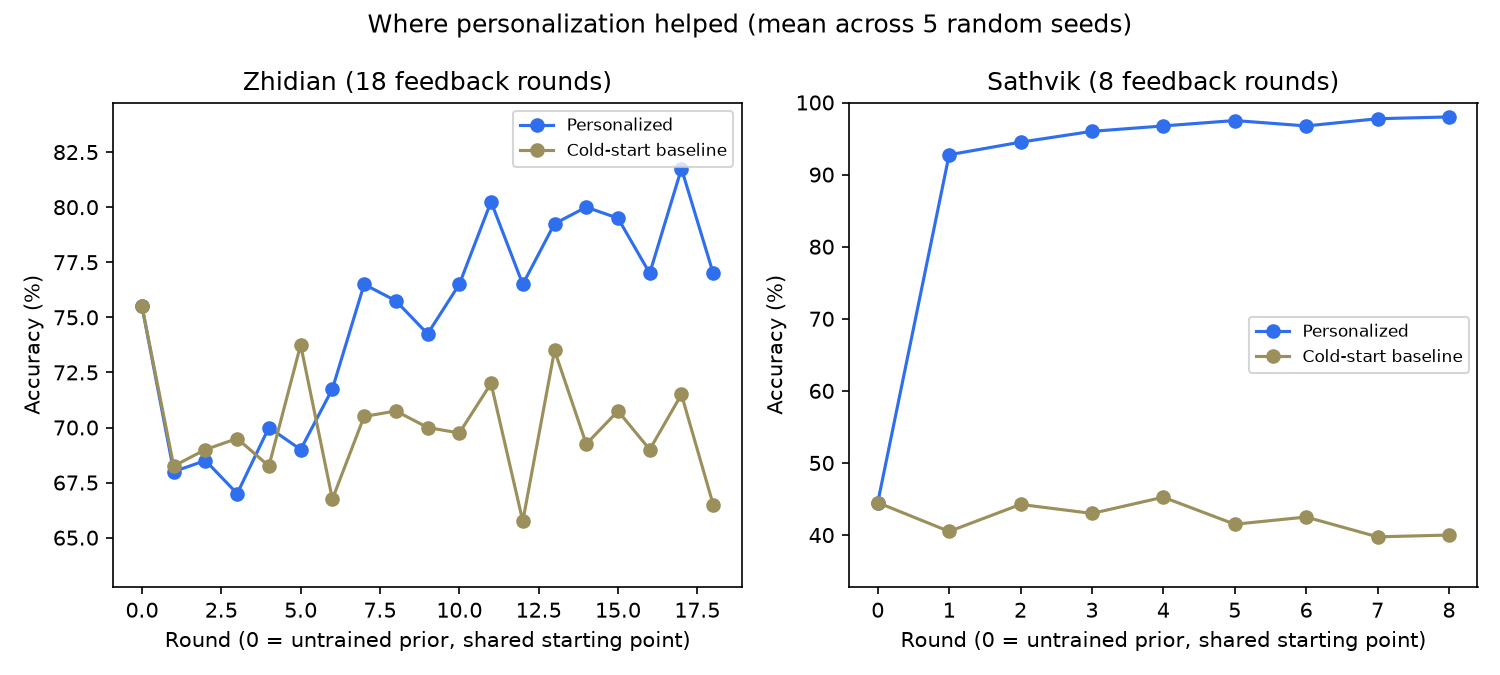
\includegraphics[width=0.9\textwidth]{figures/personalization_curve_good.png}
\caption{Datasets where personalization helped: Zhidian and Sathvik, mean across 5 random seeds. Round 0 is the shared, untrained starting point. Note the $y$-axis is zoomed to each panel's own accuracy range.}
\label{fig:curves-good}
\end{figure*}

Zhidian's dataset shows a real, if noisy, positive average lift, consistent across all five seeds tested, though individual rounds swing considerably (from $-11.2$ pp to $+23.8$ pp against the baseline within a single seed), which is expected given each round adds only 10 new labels to the accumulated history. Sathvik's dataset shows the largest lift of the three and the cleanest round-over-round rise, though it should be read with a caveat also discussed in Section~\ref{sec:analysis}: its Skip class is concentrated in a single recurring sender, which makes it an easy case for \texttt{sender\_hist} rather than a representative estimate of lift on a more diverse inbox.

\begin{figure}[h]
\centering
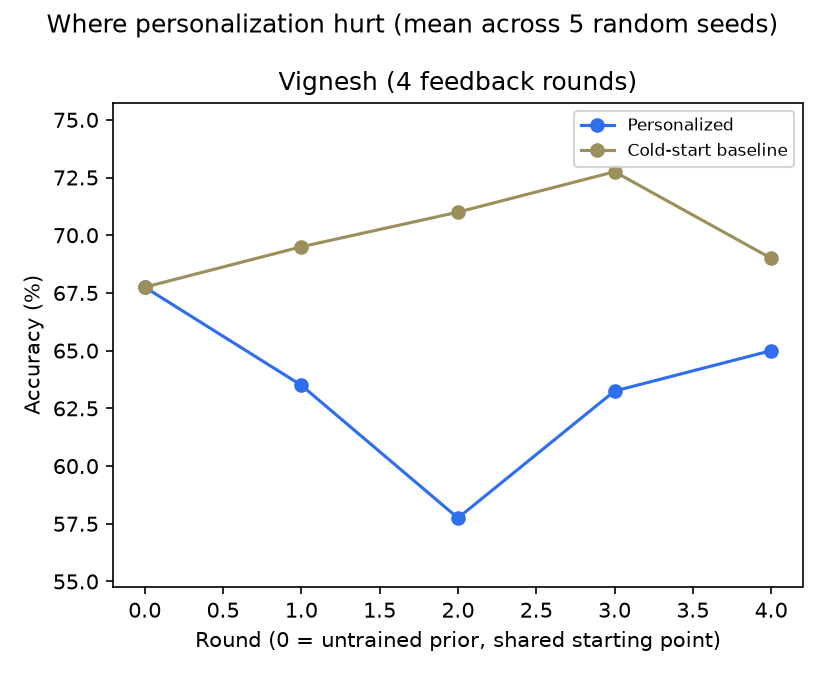
\includegraphics[width=0.5\textwidth]{figures/personalization_curve_vignesh.png}
\caption{The dataset where personalization hurt: Vignesh, mean across 5 random seeds. Round 0 is the shared, untrained starting point; personalized accuracy falls below the cold-start baseline from Round 1 onward.}
\label{fig:curves-vignesh}
\end{figure}

Vignesh's smaller dataset shows the opposite result, also consistent across all five seeds: personalization \emph{reduced} accuracy relative to the frozen prior on every seed tested. Section~\ref{sec:analysis} analyzes why: the true Keep/Skip signal in this dataset is a semantic judgment (job-role relevance) that none of our structural features represent, so the online update has no correct signal to converge to.

\textbf{Enron cold-start sanity check.} Scoring the live 18-feature prior against all 30{,}000 Enron rows with no training gives overall accuracy 0.561 (precision 0.538, recall 0.858) -- modestly above chance. As detailed in Section~\ref{sec:data}, five features are untestable on this specific Enron release, and \texttt{personalized\_greeting} tests in the wrong direction due to Enron's sent-vs-received class mismatch.

\textbf{Hand-crafted model vs. the Claude API alternative.} Table~\ref{tab:llm} reports the comparison described in the Experimental Setup, on the identical 70/30 split of Zhidian's 193-email dataset.

\begin{table}[h]
\centering
\caption{Accuracy, precision, recall, and F1 on the identical 58-email held-out test split.}
\label{tab:llm}
\resizebox{\columnwidth}{!}{%
\begin{tabular}{@{}lcccc@{}}
\toprule
\textbf{Method} & \textbf{Accuracy} & \textbf{Precision} & \textbf{Recall} & \textbf{F1} \\
\midrule
Hand-crafted & 0.879 & 0.765 & 0.812 & 0.788 \\
Claude Haiku 4.5 & 0.741 & 0.516 & 1.000 & 0.681 \\
\bottomrule
\end{tabular}%
}
\end{table}

The Claude-based classifier caught every genuinely important email in the test set (recall 1.000) but at a substantial precision cost (0.516), overshooting the hand-crafted model's already recall-weighted design (Section~\ref{sec:analysis}); its lower F1 (0.681 vs. 0.788) shows this is not simply a precision/recall trade-off in the hand-crafted model's favor -- it is a lower harmonic-mean balance of the two overall. We measured, rather than estimated, the deployment cost of the LLM alternative: two real API calls (one profile-generation call, one batch-classification call covering all 58 test emails in a single request) consumed 25{,}339 input tokens and 1{,}864 output tokens, for a total cost of \$0.035 at Claude Haiku 4.5 pricing (\$1.00 / \$5.00 per million input/output tokens), with a combined latency of 17.6 seconds -- a real, non-zero marginal cost per classification batch that the fully local hand-crafted model does not carry.

\textbf{Could we have done better?} Two opportunities we identified but did not pursue, given project scope, are testing a larger Claude model tier and collecting more per-user data before generalizing the small-dataset negative-lift finding (Table~\ref{tab:lift}) -- both discussed further in Section~\ref{sec:conclusion}.

\section{Conclusion and Future Work}
\label{sec:conclusion}

Across three real, independently collected labeled inboxes, a small, hand-designed 18-feature logistic regression with online, prior-anchored personalization outperformed both a corpus-mined-feature variant and a general-purpose LLM classifier on measured, held-out accuracy, while remaining fully local, millisecond-fast, and directly explainable. The central finding is that neither ``a well-tuned universal prior'' nor ``personalization'' can be assumed to work in general: a prior that is reasonable on average can fail completely for an individual user with different but legitimate preferences, and online personalization itself measurably helped on one real dataset and measurably hurt on a smaller one, most likely because too little accumulated feedback gave the anchored gradient descent nothing reliable to work from.

For someone wanting to use this specific solution today, we would recommend the hand-crafted local model over the LLM-based alternative: it is free to run, requires no third-party data sharing, and was measurably more accurate on our real data, at the cost of needing a modicum of hand engineering that the LLM path avoids. We would recommend collecting at least on the order of 100 labeled examples with a genuine mix of both classes before trusting the personalization mechanism, since our evidence suggests it can actively hurt below that regime; with substantially more data per user, the natural next step would be characterizing exactly where that threshold lies and re-testing whether a larger LLM tier closes the accuracy gap at an acceptable cost.

A company seeking to deploy a system like this at a large scale should weigh the same trade-off we measured directly: the hand-crafted local model has zero marginal inference cost and needs no third-party API calls, which matters enormously once inference volume reaches millions of classifications, whereas the LLM-based alternative -- despite requiring no per-feature engineering -- carries a real, measured per-batch dollar cost and network latency that scales linearly with usage and depends on sending user content to an external service. We would recommend the hand-crafted approach as the default at scale, reserving an LLM-based tier, if offered at all, for an explicitly opt-in premium feature where users knowingly accept that trade-off in exchange for zero feature-engineering effort and potentially higher recall.

\section{AI Prompts Used}

Claude (via Claude Code) was used throughout development, debugging, and analysis. The complete prompt log is in the repository as \texttt{PROMPTS\_LOG.md}; two representative prompts are quoted verbatim below, with the rest summarized by category.

\textbf{Coding.} Implementing new features in \texttt{feature\_vector()}; the Enron labeling/TF-IDF scripts (\texttt{backend/enron/}); the two-stage Claude-API classifier (\texttt{backend/llm\_eval/}); and the figure-generation script (\texttt{backend/gmail\_eval/}). Representative prompt, which led directly to \texttt{backend/llm\_eval/claude\_classify.py} and to the methodological finding in Section~\ref{sec:analysis} that an informal in-chat estimate had overstated the LLM's real accuracy: \textit{``写一个用llm 调用claude api的版本试试，因为好像效果很好，我实际测试一下体验感受''} (``build a version that actually calls the Claude API to test the LLM approach for real, since the earlier in-chat estimate looked promising'').

\textbf{Debugging.} Diagnosing the \texttt{is\_bulk\_header} cold-start issue on a job-hunting user's inbox, and inspecting the retrained Enron-prior weights that surfaced the \texttt{authority\_sender}/\texttt{system\_sender} sign problem (Section~\ref{sec:analysis}).

\textbf{Explanations.} Explaining how the hand-crafted feature/logistic-regression pipeline and the Claude-API two-call algorithm each work end to end, including cost and latency. Representative prompt: \textit{``目前调用llm的算法具体是怎么做的？''} (``how exactly does the current LLM-calling algorithm work?'').

\textbf{Research and evaluation design.} Designing the cold-start-vs-personalized comparison; a literature search for the Related Work and Related Implementations sections; and a request to re-test the LLM approach with a real API call rather than an earlier informal estimate, which turned out to have substantially overstated accuracy (Section~\ref{sec:analysis}).

\section{Declaration}
\fontsize{11}{13}\selectfont

\textbf{Conflict of Interest:} The authors declare no conflict of interest.

\textbf{Author Contribution (Statement of Contributions):}

\textbf{Zhidian Wang} -- Conceptualization, Methodology, Software, Formal Analysis, Investigation, Writing (Original Draft \& Review/Editing). Designed the core multi-feature classification algorithm and online personalization mechanism (\texttt{backend/app.py}); led testing and evaluation across the project, including the Claude-API-based classifier comparison (\texttt{backend/llm\_eval/}) and the personalization learning-curve experiments (\texttt{backend/gmail\_eval/}); wrote this report. Collected and labeled a real Gmail dataset (200 emails) used throughout these evaluations.

\textbf{Sathvik Reddy Cheruku} -- Software (Frontend \& Backend). Built the frontend interface tools (\texttt{email\_extractor.html}, \texttt{email\_priority\_demo.html}, \texttt{email\_priority\_test.html}) and contributed supporting backend work. Collected and labeled a real Gmail dataset (100 emails), which showed the largest measured personalization lift of the three datasets (Section~\ref{sec:results}).

\textbf{Vignesh Tirumani} -- Software, Formal Analysis, Investigation. Designed, implemented, and evaluated the Enron TF-IDF pretraining exploration (\texttt{backend/enron/}) -- the term-mining approach later found not to generalize and replaced by the hand-crafted structural features (Section~\ref{sec:analysis}). Collected and labeled a real Gmail dataset (60 emails); this dataset's job-hunting-related labeling pattern is analyzed as a real-data finding in the same section.

\printbibliography

\section*{\MakeUppercase{Appendix}}
\fontsize{11}{13}\selectfont

Code repository: \url{https://github.com/Shdityr/CS6140_email_priority}. See \texttt{README.md} for full installation and setup instructions (dependencies, environment setup, and commands to reproduce each experiment in Sections~\ref{sec:setup}--\ref{sec:results}). The scripts that produce this report's figures are under \texttt{backend/gmail\_eval/}; the figures themselves are under \texttt{figures/}.

\end{document}
